% Options for packages loaded elsewhere
\PassOptionsToPackage{unicode}{hyperref}
\PassOptionsToPackage{hyphens}{url}
%
\documentclass[
]{article}
\usepackage{lmodern}
\usepackage{amssymb,amsmath}
\usepackage{ifxetex,ifluatex}
\ifnum 0\ifxetex 1\fi\ifluatex 1\fi=0 % if pdftex
  \usepackage[T1]{fontenc}
  \usepackage[utf8]{inputenc}
  \usepackage{textcomp} % provide euro and other symbols
\else % if luatex or xetex
  \usepackage{unicode-math}
  \defaultfontfeatures{Scale=MatchLowercase}
  \defaultfontfeatures[\rmfamily]{Ligatures=TeX,Scale=1}
\fi
% Use upquote if available, for straight quotes in verbatim environments
\IfFileExists{upquote.sty}{\usepackage{upquote}}{}
\IfFileExists{microtype.sty}{% use microtype if available
  \usepackage[]{microtype}
  \UseMicrotypeSet[protrusion]{basicmath} % disable protrusion for tt fonts
}{}
\makeatletter
\@ifundefined{KOMAClassName}{% if non-KOMA class
  \IfFileExists{parskip.sty}{%
    \usepackage{parskip}
  }{% else
    \setlength{\parindent}{0pt}
    \setlength{\parskip}{6pt plus 2pt minus 1pt}}
}{% if KOMA class
  \KOMAoptions{parskip=half}}
\makeatother
\usepackage{xcolor}
\IfFileExists{xurl.sty}{\usepackage{xurl}}{} % add URL line breaks if available
\IfFileExists{bookmark.sty}{\usepackage{bookmark}}{\usepackage{hyperref}}
\hypersetup{
  pdftitle={Funciones de probabilidad para Diseño de Experimentos},
  pdfauthor={Diana Laura Javier Garcia},
  hidelinks,
  pdfcreator={LaTeX via pandoc}}
\urlstyle{same} % disable monospaced font for URLs
\usepackage[margin=1in]{geometry}
\usepackage{color}
\usepackage{fancyvrb}
\newcommand{\VerbBar}{|}
\newcommand{\VERB}{\Verb[commandchars=\\\{\}]}
\DefineVerbatimEnvironment{Highlighting}{Verbatim}{commandchars=\\\{\}}
% Add ',fontsize=\small' for more characters per line
\usepackage{framed}
\definecolor{shadecolor}{RGB}{248,248,248}
\newenvironment{Shaded}{\begin{snugshade}}{\end{snugshade}}
\newcommand{\AlertTok}[1]{\textcolor[rgb]{0.94,0.16,0.16}{#1}}
\newcommand{\AnnotationTok}[1]{\textcolor[rgb]{0.56,0.35,0.01}{\textbf{\textit{#1}}}}
\newcommand{\AttributeTok}[1]{\textcolor[rgb]{0.77,0.63,0.00}{#1}}
\newcommand{\BaseNTok}[1]{\textcolor[rgb]{0.00,0.00,0.81}{#1}}
\newcommand{\BuiltInTok}[1]{#1}
\newcommand{\CharTok}[1]{\textcolor[rgb]{0.31,0.60,0.02}{#1}}
\newcommand{\CommentTok}[1]{\textcolor[rgb]{0.56,0.35,0.01}{\textit{#1}}}
\newcommand{\CommentVarTok}[1]{\textcolor[rgb]{0.56,0.35,0.01}{\textbf{\textit{#1}}}}
\newcommand{\ConstantTok}[1]{\textcolor[rgb]{0.00,0.00,0.00}{#1}}
\newcommand{\ControlFlowTok}[1]{\textcolor[rgb]{0.13,0.29,0.53}{\textbf{#1}}}
\newcommand{\DataTypeTok}[1]{\textcolor[rgb]{0.13,0.29,0.53}{#1}}
\newcommand{\DecValTok}[1]{\textcolor[rgb]{0.00,0.00,0.81}{#1}}
\newcommand{\DocumentationTok}[1]{\textcolor[rgb]{0.56,0.35,0.01}{\textbf{\textit{#1}}}}
\newcommand{\ErrorTok}[1]{\textcolor[rgb]{0.64,0.00,0.00}{\textbf{#1}}}
\newcommand{\ExtensionTok}[1]{#1}
\newcommand{\FloatTok}[1]{\textcolor[rgb]{0.00,0.00,0.81}{#1}}
\newcommand{\FunctionTok}[1]{\textcolor[rgb]{0.00,0.00,0.00}{#1}}
\newcommand{\ImportTok}[1]{#1}
\newcommand{\InformationTok}[1]{\textcolor[rgb]{0.56,0.35,0.01}{\textbf{\textit{#1}}}}
\newcommand{\KeywordTok}[1]{\textcolor[rgb]{0.13,0.29,0.53}{\textbf{#1}}}
\newcommand{\NormalTok}[1]{#1}
\newcommand{\OperatorTok}[1]{\textcolor[rgb]{0.81,0.36,0.00}{\textbf{#1}}}
\newcommand{\OtherTok}[1]{\textcolor[rgb]{0.56,0.35,0.01}{#1}}
\newcommand{\PreprocessorTok}[1]{\textcolor[rgb]{0.56,0.35,0.01}{\textit{#1}}}
\newcommand{\RegionMarkerTok}[1]{#1}
\newcommand{\SpecialCharTok}[1]{\textcolor[rgb]{0.00,0.00,0.00}{#1}}
\newcommand{\SpecialStringTok}[1]{\textcolor[rgb]{0.31,0.60,0.02}{#1}}
\newcommand{\StringTok}[1]{\textcolor[rgb]{0.31,0.60,0.02}{#1}}
\newcommand{\VariableTok}[1]{\textcolor[rgb]{0.00,0.00,0.00}{#1}}
\newcommand{\VerbatimStringTok}[1]{\textcolor[rgb]{0.31,0.60,0.02}{#1}}
\newcommand{\WarningTok}[1]{\textcolor[rgb]{0.56,0.35,0.01}{\textbf{\textit{#1}}}}
\usepackage{graphicx,grffile}
\makeatletter
\def\maxwidth{\ifdim\Gin@nat@width>\linewidth\linewidth\else\Gin@nat@width\fi}
\def\maxheight{\ifdim\Gin@nat@height>\textheight\textheight\else\Gin@nat@height\fi}
\makeatother
% Scale images if necessary, so that they will not overflow the page
% margins by default, and it is still possible to overwrite the defaults
% using explicit options in \includegraphics[width, height, ...]{}
\setkeys{Gin}{width=\maxwidth,height=\maxheight,keepaspectratio}
% Set default figure placement to htbp
\makeatletter
\def\fps@figure{htbp}
\makeatother
\setlength{\emergencystretch}{3em} % prevent overfull lines
\providecommand{\tightlist}{%
  \setlength{\itemsep}{0pt}\setlength{\parskip}{0pt}}
\setcounter{secnumdepth}{-\maxdimen} % remove section numbering

\title{Funciones de probabilidad para Diseño de Experimentos}
\author{Diana Laura Javier Garcia}
\date{10/10/2020}

\begin{document}
\maketitle

\hypertarget{r-markdown}{%
\subsection{R Markdown}\label{r-markdown}}

This is an R Markdown document. Markdown is a simple formatting syntax
for authoring HTML, PDF, and MS Word documents. For more details on
using R Markdown see \url{http://rmarkdown.rstudio.com}.

When you click the \textbf{Knit} button a document will be generated
that includes both content as well as the output of any embedded R code
chunks within the document. You can embed an R code chunk like this:

4.43 Dada X una distribución normal con una media \(\mu=10\) y una
desviación estandar \(\sigma^{2}=2\). Determinar las siguientes
probabilidades.

Definición: Una variable X con función de densidad de probabilidad:

\(f(x)=\frac{1}{\sqrt{2 \pi \sigma}}e^{\frac{-(x-\mu)^{2}}{2 \sigma}}\)

Si \emph{X} es una variable aleatoria con \(E(X)=\mu\) y
\(V(X)=\sigma^{2}\), se define \emph{Z} como:
\(Z=\frac{X-\mu}{\sigma}\). Así, se tiene la forma estándar:
\(f(z)=\frac{1}{\sqrt{2 \pi }}e^{\frac{-z^{2}}{2}}\) 4.43 (a)
Probabilidades con tablas. \(\int_{x=-\infty}^{x=13} f(z) dz\)

\begin{enumerate}
\def\labelenumi{(\alph{enumi})}
\item
  P(X\textless13)=\(\int_{x=-\infty}^{x=13} f(x) dx\)
  =P(Z\textless{}\(\frac{13-10}{2}\))=P(Z\textless1.5)=0.5+0.4332=0.9332
\item
  P(X\textgreater9)=\(\int_{x=9}^{x=\infty} f(x) dx\)=P(Z\textgreater{}\(\frac{9-10}{2}\)=P(-0.5)=P(Z=0.5)+0.5=0.1915+0.5=0.6915
\item
  P(6\textless X\textless14)=\(\int_{x=6}^{x=14} f(x) dx\)=P(X\textgreater6)+P(X\textless2)=P(Z\textgreater{}\(\frac{6-10}{2}\))+P(Z\textless{}\(\frac{14-10}{2}\))=P(X\textgreater-2)+P(Z\textless2)=0.4772+0.4772=0.4544
\item
  P(2\textless X\textless4)=\(\int_{x=2}^{x=4} f(x) dx\)=P(X\textgreater2)+P(X\textless4)=P(Z\textgreater{}\(\frac{2-10}{2}\))+P(Z\textless{}\(\frac{4-10}{2}\))=P(Z\textgreater-4)+P(Z\textless-3)=0.5-0.4987=0.013
\item
  P(-2\textless X\textless8)=\(\int_{x=-2}^{x=8} f(z) dz\)=P(x\textgreater-2)+P(X\textless8)=P(X\textgreater{}\(\frac{-2+10}{2}\))+P(Z\textless{}\(\frac{8+10}{2}\))=P(Z\textgreater-1)+P(Z\textless-6)=P(Z=6)-P(Z=1)=0.5-0.3413=0.1587
\end{enumerate}

Tablas:

\begin{Shaded}
\begin{Highlighting}[]
\NormalTok{ knitr}\OperatorTok{::}\KeywordTok{include_graphics}\NormalTok{(}\StringTok{"tab1.png"}\NormalTok{)}
\end{Highlighting}
\end{Shaded}

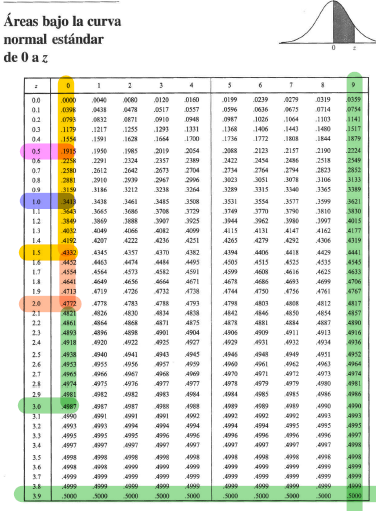
\includegraphics[width=400px]{tab1} 4.43 (b) Resultados con R:

\begin{Shaded}
\begin{Highlighting}[]
\KeywordTok{pnorm}\NormalTok{(}\DecValTok{13}\NormalTok{,}\DecValTok{10}\NormalTok{,}\DecValTok{2}\NormalTok{)}
\end{Highlighting}
\end{Shaded}

\begin{verbatim}
## [1] 0.9331928
\end{verbatim}

\begin{Shaded}
\begin{Highlighting}[]
\KeywordTok{pnorm}\NormalTok{(}\DecValTok{9}\NormalTok{,}\DecValTok{10}\NormalTok{,}\DecValTok{2}\NormalTok{,}\DataTypeTok{lower.tail =} \OtherTok{FALSE}\NormalTok{)}
\end{Highlighting}
\end{Shaded}

\begin{verbatim}
## [1] 0.6914625
\end{verbatim}

\begin{Shaded}
\begin{Highlighting}[]
\KeywordTok{pnorm}\NormalTok{(}\DecValTok{14}\NormalTok{,}\DecValTok{10}\NormalTok{,}\DecValTok{2}\NormalTok{)}\OperatorTok{-}\KeywordTok{pnorm}\NormalTok{(}\DecValTok{6}\NormalTok{,}\DecValTok{10}\NormalTok{,}\DecValTok{2}\NormalTok{)}
\end{Highlighting}
\end{Shaded}

\begin{verbatim}
## [1] 0.9544997
\end{verbatim}

\begin{Shaded}
\begin{Highlighting}[]
\KeywordTok{pnorm}\NormalTok{(}\DecValTok{4}\NormalTok{,}\DecValTok{10}\NormalTok{,}\DecValTok{2}\NormalTok{)}\OperatorTok{-}\KeywordTok{pnorm}\NormalTok{(}\DecValTok{2}\NormalTok{,}\DecValTok{10}\NormalTok{,}\DecValTok{2}\NormalTok{)}
\end{Highlighting}
\end{Shaded}

\begin{verbatim}
## [1] 0.001318227
\end{verbatim}

\begin{Shaded}
\begin{Highlighting}[]
\KeywordTok{pnorm}\NormalTok{(}\DecValTok{8}\NormalTok{,}\DecValTok{10}\NormalTok{,}\DecValTok{2}\NormalTok{)}\OperatorTok{-}\KeywordTok{pnorm}\NormalTok{(}\OperatorTok{-}\DecValTok{2}\NormalTok{,}\DecValTok{10}\NormalTok{,}\DecValTok{2}\NormalTok{)}
\end{Highlighting}
\end{Shaded}

\begin{verbatim}
## [1] 0.1586553
\end{verbatim}

\textbf{4.44 Si \emph{X} es variable con distribución normal con media
\(\mu=10\) y desviación estandar \(\sigma=2\). Determine el valor x para
el cual se cumple lo siguiente}

4.44 (a) Solución con tablas

\begin{enumerate}
\def\labelenumi{(\alph{enumi})}
\item
  P(Z\textgreater x)=0.5 =\textgreater{} P(Z=0)=0.5 =\textgreater{}
  \(z=\frac{x-10}{2}=0\) =\textgreater{} x=10\textbackslash{}
\item
  P(X\textgreater x)=0.95 =\textgreater{} P(Z=-1.645)=\textgreater0.95
  =\textgreater{} \(z=\frac{x-10}{2}=-1.650\) =\textgreater{}
  x=6.69\textbackslash{}
\item
  P(x\textless X\textless10)=0.2 =\textgreater{}
  P(z\textless{}\(\frac{10-10}{2}\))-P(z\textless{}\(\frac{x-10}{2}\))=P(z\textless0)-P(z\textless{}\(\frac{x-10}{2}\))=0.5-P(z\textless{}\(\frac{x-10}{2}\))=0.2
  =\textgreater{} P(z\textless{}\(\frac{x-10}{2}\))=-0.2+0.5=0.3
  =\textgreater{} \(z=\frac{x-10}{2}=-0.52\) =\textgreater{} x=8.96
\item
  P(-x\textless X-10\textless x)=0.95
\end{enumerate}

Resolviendo la desigualdad:
P(-x\textless X-10\textless x)=P(-x+10\textless X\textless x+10)=0.950=-P(\(\frac{(-x+10)-10}{2}\)\textless z)+P(\(\frac{(x+10)-10}{2}\))\textless z)

P(\(\frac{(-x+10)-10}{2}\)\textless z)=P(\$\frac{-x}{2}\textless z)=

4.44 (b) Solución con R

\begin{Shaded}
\begin{Highlighting}[]
\KeywordTok{qnorm}\NormalTok{(}\FloatTok{0.5}\NormalTok{,}\DecValTok{10}\NormalTok{,}\DecValTok{2}\NormalTok{)}
\end{Highlighting}
\end{Shaded}

\begin{verbatim}
## [1] 10
\end{verbatim}

\begin{Shaded}
\begin{Highlighting}[]
\KeywordTok{qnorm}\NormalTok{(}\FloatTok{0.95}\NormalTok{,}\DecValTok{10}\NormalTok{,}\DecValTok{2}\NormalTok{,}\DataTypeTok{lower.tail =} \OtherTok{FALSE}\NormalTok{)}
\end{Highlighting}
\end{Shaded}

\begin{verbatim}
## [1] 6.710293
\end{verbatim}

\begin{Shaded}
\begin{Highlighting}[]
\KeywordTok{qnorm}\NormalTok{(}\FloatTok{0.3}\NormalTok{,}\DecValTok{10}\NormalTok{,}\DecValTok{2}\NormalTok{)}
\end{Highlighting}
\end{Shaded}

\begin{verbatim}
## [1] 8.951199
\end{verbatim}

**4.60 El peso de corredor esta distribuido normalmente con una media de
12 onza y una desviación estandar de 0.5 onzas.

(a)¿Cuál es la probabilidad de que el peso sea de más de 13 onzas? Se
debe resolver lo siguiente:

P(x\textgreater13)=\(\int_{x=-\infty}^{x=13} f(x) dx\)

=P(Z\textless{}\(\frac{13-12}{0.5}\))=

\end{document}
